% Options for packages loaded elsewhere
\PassOptionsToPackage{unicode}{hyperref}
\PassOptionsToPackage{hyphens}{url}
%
\documentclass[
]{article}
\usepackage{amsmath,amssymb}
\usepackage{iftex}
\ifPDFTeX
  \usepackage[T1]{fontenc}
  \usepackage[utf8]{inputenc}
  \usepackage{textcomp} % provide euro and other symbols
\else % if luatex or xetex
  \usepackage{unicode-math} % this also loads fontspec
  \defaultfontfeatures{Scale=MatchLowercase}
  \defaultfontfeatures[\rmfamily]{Ligatures=TeX,Scale=1}
\fi
\usepackage{lmodern}
\ifPDFTeX\else
  % xetex/luatex font selection
\fi
% Use upquote if available, for straight quotes in verbatim environments
\IfFileExists{upquote.sty}{\usepackage{upquote}}{}
\IfFileExists{microtype.sty}{% use microtype if available
  \usepackage[]{microtype}
  \UseMicrotypeSet[protrusion]{basicmath} % disable protrusion for tt fonts
}{}
\makeatletter
\@ifundefined{KOMAClassName}{% if non-KOMA class
  \IfFileExists{parskip.sty}{%
    \usepackage{parskip}
  }{% else
    \setlength{\parindent}{0pt}
    \setlength{\parskip}{6pt plus 2pt minus 1pt}}
}{% if KOMA class
  \KOMAoptions{parskip=half}}
\makeatother
\usepackage{xcolor}
\usepackage[margin=1in]{geometry}
\usepackage{color}
\usepackage{fancyvrb}
\newcommand{\VerbBar}{|}
\newcommand{\VERB}{\Verb[commandchars=\\\{\}]}
\DefineVerbatimEnvironment{Highlighting}{Verbatim}{commandchars=\\\{\}}
% Add ',fontsize=\small' for more characters per line
\usepackage{framed}
\definecolor{shadecolor}{RGB}{248,248,248}
\newenvironment{Shaded}{\begin{snugshade}}{\end{snugshade}}
\newcommand{\AlertTok}[1]{\textcolor[rgb]{0.94,0.16,0.16}{#1}}
\newcommand{\AnnotationTok}[1]{\textcolor[rgb]{0.56,0.35,0.01}{\textbf{\textit{#1}}}}
\newcommand{\AttributeTok}[1]{\textcolor[rgb]{0.13,0.29,0.53}{#1}}
\newcommand{\BaseNTok}[1]{\textcolor[rgb]{0.00,0.00,0.81}{#1}}
\newcommand{\BuiltInTok}[1]{#1}
\newcommand{\CharTok}[1]{\textcolor[rgb]{0.31,0.60,0.02}{#1}}
\newcommand{\CommentTok}[1]{\textcolor[rgb]{0.56,0.35,0.01}{\textit{#1}}}
\newcommand{\CommentVarTok}[1]{\textcolor[rgb]{0.56,0.35,0.01}{\textbf{\textit{#1}}}}
\newcommand{\ConstantTok}[1]{\textcolor[rgb]{0.56,0.35,0.01}{#1}}
\newcommand{\ControlFlowTok}[1]{\textcolor[rgb]{0.13,0.29,0.53}{\textbf{#1}}}
\newcommand{\DataTypeTok}[1]{\textcolor[rgb]{0.13,0.29,0.53}{#1}}
\newcommand{\DecValTok}[1]{\textcolor[rgb]{0.00,0.00,0.81}{#1}}
\newcommand{\DocumentationTok}[1]{\textcolor[rgb]{0.56,0.35,0.01}{\textbf{\textit{#1}}}}
\newcommand{\ErrorTok}[1]{\textcolor[rgb]{0.64,0.00,0.00}{\textbf{#1}}}
\newcommand{\ExtensionTok}[1]{#1}
\newcommand{\FloatTok}[1]{\textcolor[rgb]{0.00,0.00,0.81}{#1}}
\newcommand{\FunctionTok}[1]{\textcolor[rgb]{0.13,0.29,0.53}{\textbf{#1}}}
\newcommand{\ImportTok}[1]{#1}
\newcommand{\InformationTok}[1]{\textcolor[rgb]{0.56,0.35,0.01}{\textbf{\textit{#1}}}}
\newcommand{\KeywordTok}[1]{\textcolor[rgb]{0.13,0.29,0.53}{\textbf{#1}}}
\newcommand{\NormalTok}[1]{#1}
\newcommand{\OperatorTok}[1]{\textcolor[rgb]{0.81,0.36,0.00}{\textbf{#1}}}
\newcommand{\OtherTok}[1]{\textcolor[rgb]{0.56,0.35,0.01}{#1}}
\newcommand{\PreprocessorTok}[1]{\textcolor[rgb]{0.56,0.35,0.01}{\textit{#1}}}
\newcommand{\RegionMarkerTok}[1]{#1}
\newcommand{\SpecialCharTok}[1]{\textcolor[rgb]{0.81,0.36,0.00}{\textbf{#1}}}
\newcommand{\SpecialStringTok}[1]{\textcolor[rgb]{0.31,0.60,0.02}{#1}}
\newcommand{\StringTok}[1]{\textcolor[rgb]{0.31,0.60,0.02}{#1}}
\newcommand{\VariableTok}[1]{\textcolor[rgb]{0.00,0.00,0.00}{#1}}
\newcommand{\VerbatimStringTok}[1]{\textcolor[rgb]{0.31,0.60,0.02}{#1}}
\newcommand{\WarningTok}[1]{\textcolor[rgb]{0.56,0.35,0.01}{\textbf{\textit{#1}}}}
\usepackage{graphicx}
\makeatletter
\def\maxwidth{\ifdim\Gin@nat@width>\linewidth\linewidth\else\Gin@nat@width\fi}
\def\maxheight{\ifdim\Gin@nat@height>\textheight\textheight\else\Gin@nat@height\fi}
\makeatother
% Scale images if necessary, so that they will not overflow the page
% margins by default, and it is still possible to overwrite the defaults
% using explicit options in \includegraphics[width, height, ...]{}
\setkeys{Gin}{width=\maxwidth,height=\maxheight,keepaspectratio}
% Set default figure placement to htbp
\makeatletter
\def\fps@figure{htbp}
\makeatother
\setlength{\emergencystretch}{3em} % prevent overfull lines
\providecommand{\tightlist}{%
  \setlength{\itemsep}{0pt}\setlength{\parskip}{0pt}}
\setcounter{secnumdepth}{-\maxdimen} % remove section numbering
\usepackage{booktabs}
\usepackage{longtable}
\usepackage{array}
\usepackage{multirow}
\usepackage{wrapfig}
\usepackage{float}
\usepackage{colortbl}
\usepackage{pdflscape}
\usepackage{tabu}
\usepackage{threeparttable}
\usepackage{threeparttablex}
\usepackage[normalem]{ulem}
\usepackage{makecell}
\usepackage{xcolor}
\ifLuaTeX
  \usepackage{selnolig}  % disable illegal ligatures
\fi
\IfFileExists{bookmark.sty}{\usepackage{bookmark}}{\usepackage{hyperref}}
\IfFileExists{xurl.sty}{\usepackage{xurl}}{} % add URL line breaks if available
\urlstyle{same}
\hypersetup{
  pdftitle={Introduction to hydroGraphR},
  pdfauthor={Paula Soto },
  hidelinks,
  pdfcreator={LaTeX via pandoc}}

\title{Introduction to hydroGraphR}
\author{Paula Soto}
\date{2025-03-05}

\begin{document}
\maketitle

\texttt{hydroGraphR} is an R package designed to simplify the process of
creating hydrographs that compare historical hydrometric data with a
specific year's traces. This vignette provides an overview of the
package's functionality and demonstrates how to use it in a typical
workflow.

\hypertarget{installation}{%
\subsection{Installation}\label{installation}}

To install the development version of \texttt{hydroGraphR} from GitHub:

\begin{Shaded}
\begin{Highlighting}[]
\CommentTok{\# Install devtools if not already installed}
\FunctionTok{install.packages}\NormalTok{(}\StringTok{"devtools"}\NormalTok{)}

\FunctionTok{library}\NormalTok{(devtools)}

\CommentTok{\# Install hydroGraphR}
\FunctionTok{install\_github}\NormalTok{(}\StringTok{"pausoto7/hydroGraphR"}\NormalTok{)}

\CommentTok{\# Download library}
\FunctionTok{library}\NormalTok{(hydroGraphR)}
\end{Highlighting}
\end{Shaded}

\hypertarget{workflow-overview}{%
\subsection{Workflow Overview}\label{workflow-overview}}

A typical workflow for hydroGraphR involves the following steps:

\begin{enumerate}
\def\labelenumi{\arabic{enumi}.}
\tightlist
\item
  Download hydrometric data for specific WSC stations.
\item
  Generate single-year and historical statistics.
\item
  Visualize the data by creating hydrographs.
\end{enumerate}

\hypertarget{step-1-download-hydrometric-data}{%
\subsubsection{Step 1: Download Hydrometric
Data}\label{step-1-download-hydrometric-data}}

Use the \texttt{dl\_hydro()} function to download data for specific
Water Survey of Canada (WSC) station numbers. You can find station
numbers on the
\href{https://wateroffice.ec.gc.ca/search/real_time_e.html}{WSC
website}. Note that with this function historical and real time data
will be downloaded. Typically, historical data has been QAQC'd and
occurred longer than two years ago. Real time data is data collected
within the last two years and \textbf{has not} been QAQC'd.~

You may also assign nick names to stations for easier identification in
subsequent analyses. If you are going to use nick names ensure that the
number of nick names matches the number of station numbers.

Examples:

\begin{Shaded}
\begin{Highlighting}[]
\CommentTok{\#example of station(s) download without nicknames}
\NormalTok{hydro\_data }\OtherTok{\textless{}{-}} \FunctionTok{dl\_hydro}\NormalTok{(}\AttributeTok{station\_number =} \FunctionTok{c}\NormalTok{(}\StringTok{"08LD001"}\NormalTok{, }\StringTok{"08LC002"}\NormalTok{))}

\CommentTok{\#example of station(s) download with nick names. }
\NormalTok{hydro\_data\_nickname }\OtherTok{\textless{}{-}} \FunctionTok{dl\_hydro}\NormalTok{(}\AttributeTok{station\_number =} \StringTok{"08LD001"}\NormalTok{, }\AttributeTok{nick\_name =} \StringTok{"Adams River"}\NormalTok{)}
\end{Highlighting}
\end{Shaded}

\hypertarget{step-2-create-statistics-for-single-year-and-historical-data}{%
\subsubsection{Step 2: Create Statistics for Single Year and Historical
Data}\label{step-2-create-statistics-for-single-year-and-historical-data}}

Once the hydrometric data is downloaded, you can calculate statistics
for:

\begin{itemize}
\tightlist
\item
  A specific year of interest (YOI) using
  \texttt{create\_hydro\_stats\_singleYr()}.
\item
  Historical data using \texttt{create\_hydro\_stats\_historical()}.
\end{itemize}

Statistics calculated are listed in more detail in Step 3.

WY is a logical value indicating whether to present hydrograph by water
year (Nov-Oct) (TRUE) or calendar year (Jan-Dec) (FALSE).

Max/min dates can also be selected for historical dates if focus is on a
specific period.For example, you could enter date\_minimum =
``2010-01-01'', date\_maximum - ``2019-12-31'' and YOI = 2020 if you
wanted to compare 2020 with the 2010's.

\textbf{\emph{Important Note: Data from the past two years may be
provisional, as such should be used with caution when a recent YOI is
selected. Status of data can be found on the WSC website.}}

\begin{Shaded}
\begin{Highlighting}[]
\NormalTok{all\_hydro\_sites\_1yr }\OtherTok{\textless{}{-}} \FunctionTok{create\_hydro\_stats\_singleYr}\NormalTok{(hydro\_data, }
                                                   \AttributeTok{YOI =} \DecValTok{2021}\NormalTok{, }
                                                   \AttributeTok{WY =} \ConstantTok{FALSE}\NormalTok{) }\CommentTok{\# Calendar year}

\NormalTok{all\_hydro\_sites\_hist }\OtherTok{\textless{}{-}} \FunctionTok{create\_hydro\_stats\_historical}\NormalTok{(hydro\_data) }\CommentTok{\# Use all available hydrometric data}
\end{Highlighting}
\end{Shaded}

\hypertarget{step-3-create-hydrographs}{%
\subsubsection{Step 3: Create
Hydrographs}\label{step-3-create-hydrographs}}

Visualize your data using one of two functions, depending on your
preferred output style.

\begin{itemize}
\item
  \texttt{create\_hydrograph\_separate()}- Generates individual
  hydrographs for each station.
\item
  \texttt{create\_hydrograph\_faceted()} - Creates a single faceted plot
  displaying multiple stations together.
\end{itemize}

Variables shown on hydrograph legends are described here:

Term

Definition

YOI

Mean

The average value of the measurements over the YOI period.

Historical

Mean

The average value of the measurements over the historical period.

Q25 (Today)

The 25th percentile of today's data distribution, indicating that 25\%
of the data points are below this value.

Q75 (Today)

The 75th percentile of today's data distribution, indicating that 75\%
of the data points are below this value.

MAD

Mean Annual Discharge, a measure of the average amount of discharge
through a river or stream over the course of a year.

Date Ranges

The years during which the data was collected and included in analysis.

\hypertarget{variables}{%
\paragraph{Variables}\label{variables}}

\begin{itemize}
\item
  \textbf{Parameter}: Options are \texttt{"flow"} for a discharge
  hydrograph, and \texttt{"level"} for a water level hydrograph.
\item
  \textbf{WY}: Logical value indicating whether to present hydrograph by
  water year (Nov-Oct)(\texttt{TRUE}) or calendar year
  (Jan-Dec)(\texttt{FALSE}).

  \begin{itemize}
  \tightlist
  \item
    No matter the output selection ensure that the water year (WY)
    choice matches the selection made in Step 2. For example, if
    ``calendar year'' was chosen for statistics in Step 2, it must also
    be selected for the hydrograph presentation. Selecting a different
    year type will result in missing data on the hydrograph and trigger
    a warning.
  \end{itemize}
\item
  \textbf{output\_type}:

  \begin{itemize}
  \tightlist
  \item
    \texttt{"print"} will print your image in R, useful for embedding in
    rmarkdown or shiny type outputs.
  \item
    \texttt{"jpeg"} will produce a jpeg image and save it to the
    ``figures/'' folder of this project.
  \end{itemize}
\end{itemize}

\hypertarget{option-1-create_hydrograph_separate}{%
\paragraph{\texorpdfstring{\textbf{Option 1}:
\texttt{create\_hydrograph\_separate()}}{Option 1: create\_hydrograph\_separate()}}\label{option-1-create_hydrograph_separate}}

\begin{itemize}
\tightlist
\item
  This function creates separate hydrographs as individual images which
  are ideal for standalone use or printing. When the ``jpeg'' option is
  selected in this option, an additional title will appear on the image
  with the station name to avoid confusion of station ID if the file
  name is not easily available (for example if the image is pasted into
  a word document).
\end{itemize}

\begin{Shaded}
\begin{Highlighting}[]

\FunctionTok{create\_hydrograph\_separate}\NormalTok{(}
\NormalTok{  all\_hydro\_sites\_hist,}
\NormalTok{  all\_hydro\_sites\_1yr,}
  \AttributeTok{parameter =} \StringTok{"flow"}\NormalTok{, }\CommentTok{\# Discharge hydrograph}
  \AttributeTok{output\_type =} \StringTok{"print"}\NormalTok{,}
  \AttributeTok{WY =} \ConstantTok{FALSE} \CommentTok{\# calendar year}
\NormalTok{)}
\end{Highlighting}
\end{Shaded}

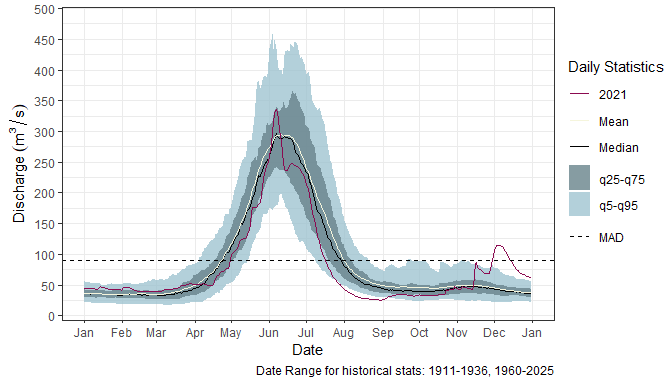
\includegraphics{README_files/figure-latex/hydrographsep-1.pdf}
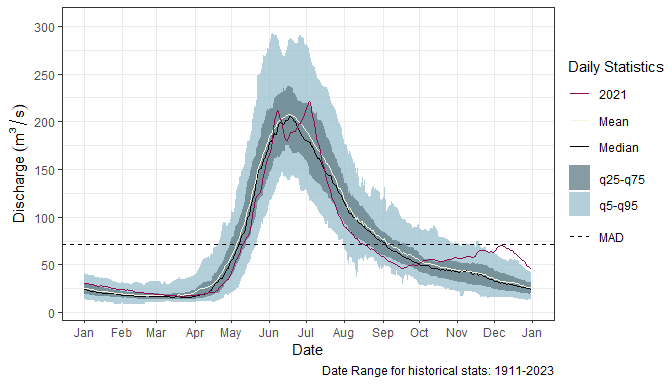
\includegraphics{README_files/figure-latex/hydrographsep-2.pdf}

\hypertarget{option-2-create_hydrograph_faceted}{%
\paragraph{\texorpdfstring{\textbf{Option 2}:
\texttt{create\_hydrograph\_faceted()}}{Option 2: create\_hydrograph\_faceted()}}\label{option-2-create_hydrograph_faceted}}

\begin{itemize}
\item
  This function creates a single faceted hydrograph, making it easy to
  compare multiple stations side by side. There are a few additional
  variabels that can also be modified in this function:

  \begin{itemize}
  \tightlist
  \item
    \texttt{fixed\_y\_scales}: A character string specifying whether the
    y-axis scale is ``fixed'' or ``free'' across facets. Defaults to
    ``fixed''.
  \item
    \texttt{custom\_ymax\_input}: A numeric value for a custom maximum
    y-axis value. Leave as NA for automatic ymax.
  \item
    \texttt{custom\_ymin\_input}:A numeric value for a custom minimum
    y-axis value. Leave as NA for automatic ymin.
  \item
    \texttt{jpeg\_width}: A numeric value specifying the width of the
    figure (in inches) for JPEG output. 6 inches is automatic output.\\
  \item
    \texttt{jpeg\_height}: A numeric value specifying the height of the
    figure (in inches) for JPEG output. 8 inches is automatic output.
  \end{itemize}
\end{itemize}

\begin{Shaded}
\begin{Highlighting}[]

\FunctionTok{create\_hydrograph\_faceted}\NormalTok{(}
\NormalTok{  all\_hydro\_sites\_hist,}
\NormalTok{  all\_hydro\_sites\_1yr,}
  \AttributeTok{parameter =} \StringTok{"flow"}\NormalTok{,}
  \AttributeTok{WY =} \ConstantTok{FALSE}\NormalTok{, }\CommentTok{\# calendar year}
  \AttributeTok{output\_type =} \StringTok{"print"}\NormalTok{, }
  \AttributeTok{fixed\_y\_scales =} \StringTok{"fixed"}\NormalTok{,}
  \AttributeTok{custom\_ymax\_input =} \ConstantTok{NA}\NormalTok{, }
  \AttributeTok{custom\_ymin\_input =} \ConstantTok{NA}
\NormalTok{)}
\end{Highlighting}
\end{Shaded}

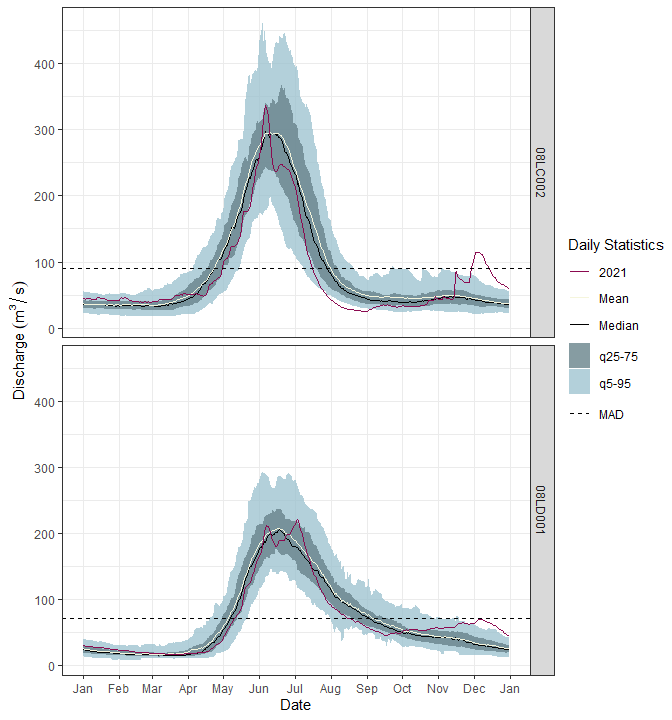
\includegraphics{README_files/figure-latex/hydrofacet-1.pdf}

\hypertarget{additional-tools}{%
\subsubsection{Additional tools}\label{additional-tools}}

You can combine these tools with other R packages to create streamlined
workflows for hydrologic data analysis. For example, the
\texttt{streamTrackR} package complements \texttt{hydroGraphR} by
enabling easy comparison of current conditions across selected rivers.

\hypertarget{summary}{%
\subsubsection{Summary}\label{summary}}

\texttt{hydroGraphR} simplifies hydrometric data analysis and
visualization with functions for downloading data, generating
statistics, and creating hydrographs. Whether working with individual
rivers or a larger dataset, the package offers flexibility for both
exploratory and presentation-ready outputs.

For further details, consult the package documentation

\end{document}
